
\section{The HMS Detector Package and Shield House }

All the detectors are in the shield house (also referred to as the detector hut,
located at the top of the
rear set of stairs). The shield house has one wall which is removable
in order to gain completely free access to the detectors. The removal
of this wall is rarely needed as there is a door that provides access
to the hut and there is adequate room inside the hut for most activities.
Essentially, the only activities that require the removal of the hut
wall are the installation or removal of an entire detector. The
hut wall may only be removed by Hall~C approved, and trained crane
operators and requires
several people. Mike Fowler, Hall~C mechanical technician,  
must be contacted if the hut wall needs to be removed.

The hut door is motorized, and must therefore be opened manually. Keep in mind when opening and closing the
shield house door that it weighs approximately 15 tons and therefore has
considerable inertia. This means that you must pull backwards on the door
in order to slow it down near the end of its desired motion.

The detector package is key to a successful measurement. Its
proper operation should therefore be constantly monitored during shifts. There
are normally a number of diagnostic spectra available to aid in this
process.  Typically each collaboration customizes it's own set of
diagnostic spectra.  

\subsection{High Voltage Supplies}

All the detector elements require the use of High Voltage. The
high voltage supplies for the detectors are located in the
electronics room of the counting house. They are connected to
the detector shield house through a multiconductor high voltage patch system,
and to the detectors through coaxial cables with SHV connectors.
During experiments the control of the high voltage supplies is
done remotely via computer and a display is available on one 
of the xterms around the console in the Hall~C counting house. The control is via
EPICS and includes a graphical display so that the status of each
HV channel can be seen at a glance. See section~\ref{par:hv_ops} for
operating instructions.

As a general rule no work should be done on detectors which are under
High Voltage and
High Voltage cables should never be removed or installed while the supply is on.
General information about the use of the {\em CAEN} power supplies can be
found in a previous Section.


\subsection{Drift Chambers}

\paragraph{Overview}

The drift chambers provide accurate measurements of the particles
position and angles in the detector hut. This information can be combined
with a knowledge of the spectrometer optics to infer the trajectory of the
particles at the target.

The planes are designated X,Y,U,V,Y$'$, and X$'$.
X and X$'$ wires measure position along the dispersive direction.
Y and Y$'$ wires measure in the transverse direction while
the U and V planes are inclined at fifteen degrees with respect to the
X planes.

In addition to High Voltage the drift chambers have amplifier discriminator
cards which require Low Voltage. These Low Voltage supplies
(built by {\em Accopian}) are
in racks in the shield house. They are not computer controlled.

The thresholds of the discriminators are held by a third set of supplies
which are located upstairs in the counting house. This control
is in the left side of the far left hand set of blue racks (near the disk drives) in the
electronics bay of the Hall~C counting house.

The amplified and discriminated signals from the chambers are fed
to the starts of {\em LeCroy} Model 1877 Fastbus pipeline TDC's. These
TDC's are located in the detector hut in an electronics rack on the
far side (from the door) of the detector mounting stand.
%The hazards associated with electronics crates are discussed in
%\cite{bi:arr95}.

The chambers are filled with a mixture of Argon, Ethane and Isopropyl Alcohol
($\approx$ 49.5 $\%$, 49.5 $\%$  and $1\%$ by weight respectively).
The gas bottles are in the bottle racks behind the gas shed. The gas shed
is located in the parking lot to the left of the counting house when one is facing the counting
house between the counting house and the accelerator
service building.  The alcohol is placed in the gas
by bubbling the gas through a refrigerated bubbler. This bubbler is
located in the gas shed.

There are gas log books that must be completed each shift.
When a bottle is near empty it should be changed.
Care should be used when handling high pressure gas bottles as the
potential energy stored in such a bottle is tremendous.
Gas bottles can only be changed by authorized personnel.

The gas mixing system is in the gas shed. The mixing is accomplished
by an electronic system. The flow rates of the gases can be read off the
LCD display of the flow meter located in the gas panel rack in the shed.
This information must be entered in the gas log book along with the bottle contents.
Only authorized personnel should make adjustments to the gas flow system.
All permanent members
of the Hall~C physics and engineering staff may change gas bottles.

As is true for all detector systems, in case you note a loss of power
during experiment conditions, check the VESDA panel in the Hall~C counting
house to see whether there is a potential fire before resetting (also
see the section on ``Fire" at the beginning of this chapter).

\paragraph {Gas Flow Operating Procedures}

The HMS drift chambers use a 50:50 mixture (by weight) of argon and
ethane gas.  Each chamber has a volume of about 120 liters.  Each is
operated slightly above atmospheric pressure.  The gas flow through
the two chambers can be varied and is typically set at 1000 cc/min
when flushing (full purge in about 2.5 hours) and 400 cc/min when operating
at low to moderate charged particle rates.  The chambers are connected
in parallel for gas flow as shown in Figure~\ref{fig:5.1}.  There are flow meters 
connected
to the exit line of each chamber.  The gas flow control electronics
and gas handling system (GHS) are located in the gas shed just outside
of the Hall~C counting house.  The gas cylinders are kept just outside of
this shed.  Both the argon and ethane cylinders have regulators (the ethane
cylinder must use a CGA-350 regulator since it is a combustible gas) for
reading the gas pressure in the bottle (high pressure) and in the line (low
pressure).  However, the ethane
in the cylinder is a liquid, so that the WEIGHT of the cylinder is important
for monitoring the amount of ethane remaining.  The ethane
cylinder sits on a 'bathroom scale' for this reason.  An empty cylinder
(standard size) weighs 110 lbs.

\begin{figure}
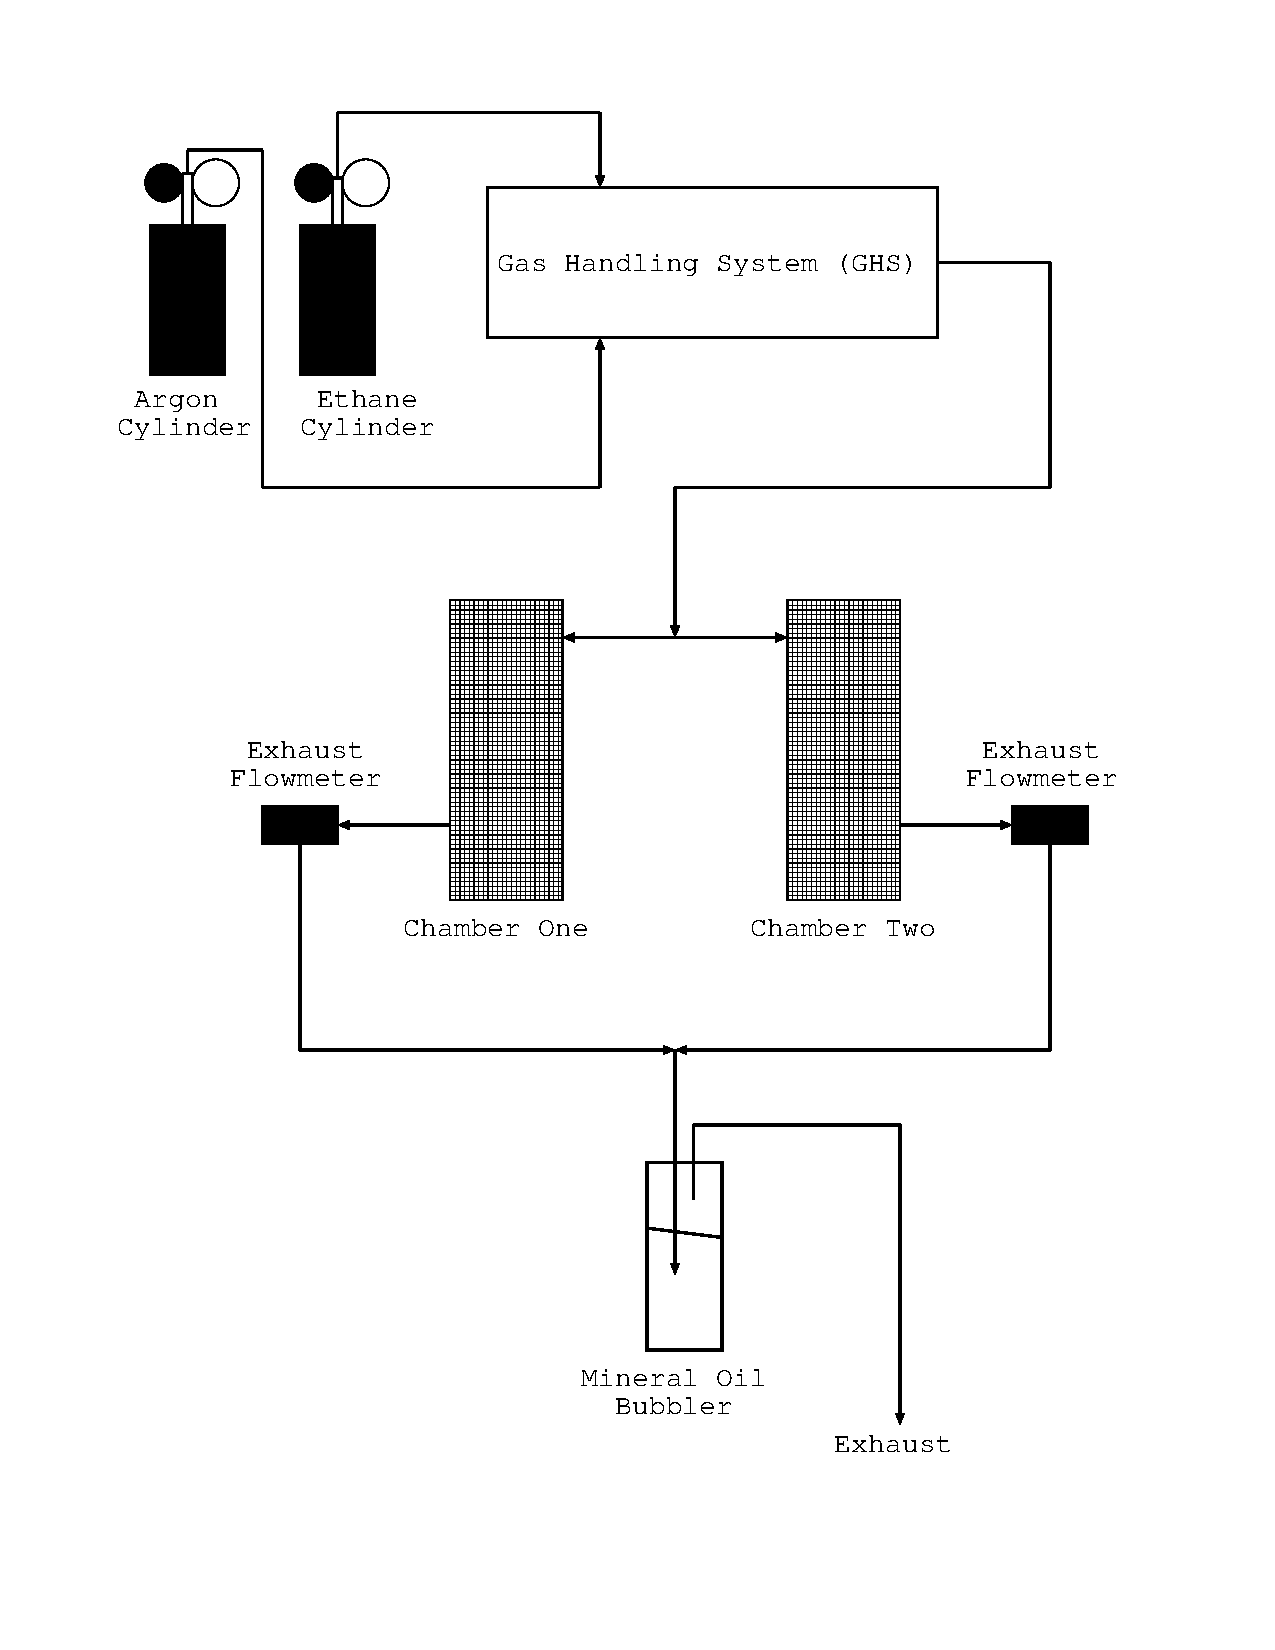
\includegraphics[height=7.5in]{HMSdriftch.pdf}
\caption{The Gas Handling System for the HMS Drift Chambers. \label{fig:5.1}}
\end{figure}

\begin{center}
{\bf Procedure}
\end{center}

\begin{enumerate}
\item {Visually check that the gas flow lines are connected to the two
HMS chambers.}
\item {Check gas pressure and amount in gas cylinders (Ar and C$_2$H$_6$).}
\item {Turn on the gas flow on the MKS controller in the gas hut.}
\item {Set flow through channels three and four to 800 sccm each
(for purging).}
\item {After about 15 minutes, the oil bubbler in the gas hut should
indicate flow.}
\item {The flow rates as read on the flow meters at the chambers should
indicate very low flow (0.3 or so).}
\end{enumerate}

The above settings are for 400 sccm flow through each chamber.  The gas
cylinders should be changed when about 90\% used.  The gas handling system
parameters should be checked every shift (see the checklist at the end of
this document).

\paragraph{Electronics Operating Procedures}

The readout electronics associated with the HMS drift chambers are all
commercial products from LeCroy Research Systems, Nanometrics, Kinetic Systems,
and BiRa Corporation.  There are 544 electronics channels per chamber for
a total of 1088 readout channels.  These anodes are read out using LRS 2735DC
and Nanometrics N-277 preamplifier/discriminator cards mounted directly
on the chambers.  Each chamber has both types of cards, however each plane
(of six total planes per chamber) has only one type of card.  The
digitized signals are sent to FASTBUS TDC inside of the detector hut
via twisted pair cable.  The low voltage (preamplifier) power supplies
(the Acopian supplies)
are in the 13 inch blue rack at the rear of the detector hut.  The
threshold voltage power supplies are on the frame under the Cerenkov
counter.  The remote
threshold power supplies are located in the electronics room of the counting
house.

\begin{center}
{\bf Procedure (in the detector hut)}
\end{center}

\begin{enumerate}
\item {Turn on low voltage power supplies (the Acopian Supplies).}
\item {Turn on threshold voltage power supply to appropriate setting.}
\item {Turn on the FASTBUS power supply if it is not already on.}
\end{enumerate}

It is important that the Acopian power supplies be turned on {\bf BEFORE} the
FASTBUS supplies or the FASTBUS crate will hang up.  The threshold voltage
can be controlled locally in the detector hut or remotely in the
counting house. There is approximately a one volt drop in the threshold
voltage line in going from upstairs in the counting house to
downstairs in the detector hut.  Hence the supplies in the counting
house should be set to 5.5 volts. The local/remote switch is on the
controller in the
detector hut.  It should be switched to remote before exiting the hut.  The
LeCroy preamp/disc cards have LEDs (a green and a red light) which indicate
that the power is delivered properly to the chamber electronics.

\paragraph{High Voltage Operating Procedures}

Only formally authorized person may alter drift chamber high voltage.
There are four different voltages per chamber which must be turned on at the
proper time and monitored throughout the experiment.  {\bf MAKE SURE THAT
GAS IS FLOWING THROUGH THE CHAMBERS AND THAT THERE ARE 
EDGE 
CARDS MOUNTED
ON ALL READOUT CHANNELS BEFORE TURNING ON HIGH VOLTAGE.}  
The high voltage
power supplies are the CAEN supplies located in relay rack CH03B17 in
the counting house electronics room.  The
voltages are set remotely using the GUI in the counting
house. See section \ref{par:hv_ops} for operating instructions.
The four different voltages are (nominally): triangle
wires (corner field wires) (-2500 V),
square wires (-2250 V), circle wires (-1800 V), and guard wires (-1500 V).
Note that each HMS drift chamber {\em plane} has its own triangle, circle,
and square voltage source, while there is only one guard wire voltage
source per {\em chamber}.
\begin{center}
{\bf Procedure (in the detector hut)}
\end{center}

\begin{enumerate}
\item {Make sure a 2735DC card or a grounding plate is on each instrumented
connector on the chamber.}
\item {Make sure that there is gas flow, particularly Ar gas.}
\item {Make sure high voltage cables are properly connected to
chamber.}
\item {Turn on high voltage, using the EPICS GUI in the counting house, 
to proper settings.}
\end{enumerate}

The CAEN power supplies, when operated remotely, are controlled by the
EPICS control system.  To operate, log on to vxworks, get the high
voltage monitors (use the rightmost mouse button to bring up the menu)
and choose the chamber voltage group.  Each high voltage channel is
independently controlled.

In general all of the voltages and gas flow should be left on, even when
no data is being collected.  The gas supply should be checked periodically,
approximately once every shift.  The gas bottles' supply is depleted
after about 2 weeks at the nominal (400 cc/min) flow rate.
In the case of a HV trip, try cycling the CAEN power supplies.  If this fails, call
one of the responsible persons listed in the Responsible Personnel Section 
of the \htmladdnormallinkfoot{ESAD}{http://www.jlab.org/Hall-C/document}.




\subsection{Scintillator Hodoscopes (HMS and SOS)}

The purpose of the scintillator hodoscopes is to provide a clean
trigger as well as particle identification by time of flight (TOF). These
detectors consist of two pairs of spatially separated scintillator
layers: a pair comprised of S1X and S1Y, and approximately 2 meters away a pair
comprised of S2X and S2Y. General characteristics of the BC404 scintillator
material are as follows:

\begin{itemize}
\item{Polyvinyltoluene (PVT) is the base material. }
\item{Light output is 68\% that of Anthracene. }
\item{Wavelength of maximum emission is 408 nm.}
\item{Decay constant of the main fluorescence component is 1.8 ns.}
\item{Bulk attenuation length is 160 cm.}
\end{itemize}

	The specific dimensions for the scintillator elements in the HMS
are found in Table~\ref{tab:tof_scintillators}.
\begin{table}
\caption{Dimensions (at 70~F.) of the scintillators for the HMS TOF system. 
\label{tab:tof_scintillators}}
\begin{center}
  \begin{tabular}{ccccc}
	&Thickness	&Width		&Length		&Number	\\
	&		&		&		&	\\
\hline
X(HMS)	&	1cm	&	8.0cm	&	75.5cm	&32 units\\
Y(HMS)	&	1cm	&	8.0cm	&	120.5cm	&20 units\\
%	&		&		&		&	\\
%X1(SOS) &       1cm     &       7.5cm   &       36.5cm  &9 units\\
%Y1(SOS) &       1cm     &       4.5cm   &       63.5cm  &9 units\\
%X2(SOS) &       1cm     &       7.5cm   &       36.5cm  &16 units\\
%Y2(SOS) &       1cm     &       4.5cm   &       112.5cm &9 units\\
  \end{tabular}
\end{center}
\end{table}
Each scintillator is read out by two Philips XP2282B photomultiplier
tubes (PMT's). These PMT's are 8-stage tubes with nominal operation at
2500 volts. The bases have two anode outputs, one of which is terminated with a
short clip line and 40 Ohms.  Because of pmt to pmt variations in gain and the
5\% precision zener diodes in the bases, the spread in gains can be a factor of
2-3. Individual high voltages must therefore be adjusted to balance the gains.
The gains have been carefully matched with a source, and HV save files exist,
so the gains will not normally need to be readjusted. If gain adjustment is
necessary, inform one of the hodoscope contact persons as soon as possible.
Mysterious gain shifts are probably due to transient problems like bad solder
contacts or broken glue joints. They require repair. A rough rule of thumb is
that an increase of 50 volts will increase the gain by 30\%.

With our base, the HV channel will trip on overcurrent (3 mA) at 2900 V
(this base is essentially divider C in the Philips catalog). If a channel needs
more than 2800 volts, and the base and glue joints are okay, then our policy
is to replace the pmt. We have several spare modules in the counting room.
In desperation, ``spares" can be taken from the edges of the acceptance. In the
HMS, S1X16 or S2X16 contain little or no useful data, and similarly for S1Y01
or S1Y10.

	The light guide material is UVT lucite.  Wrapping material for the SOS scintillator elements was one layer of 
aluminized mylar (aluminum side facing inward), followed by two layers of
tedlar for light tightness. The HMS elements were wrapped in aluminum foil,
followed by one layer of tedlar.

	The SOS hodoscopes are mounted in aluminum frames, with brackets over
the lightguides and holders supporting the elements also at the tube/base
assembly. The SOS y-counters are EXTREMELY delicate at the glue joints
connecting the angled light guide with the flat section, due to the geometry.
The HMS elements are supported at the lightguides. In case of repair use BC-600
glue. Each element has a 1 mm plastic fiber glued into the light guide. These
fibers are also very delicate and care must be taken when moving a scintillator
element to avoid snagging and breaking the fibers.

{\bf What to check}: Before starting to operate the detectors, one has to
check the trip setting (current limit) of the HV power supply for each channel
and the set HV value of each channel. During operation, the current of each
channel and its HV should be periodically checked. The HV should be on for at
least half an hour before taking data. During runs one should check the
histogram of the plane hit distribution. This should be rather flat reflecting
the normal trigger requirement of 3 out of 4 planes. Also the element hit
distributions for the individual planes should be checked regularly. These
distributions are defined for both ends of the elements using both ADC and TDC
information.

{\bf Nomenclature}:
The coordinate system (right handed, following TRANSPORT
convention) is defined as z downstream, x pointing down, and when looking
downstream, y to the left. In this convention the X-tubes at positive Y are
called X+ and the Y tubes at the bottom (pos x ) are called Y+. Numbering of
the elements is done as one would read a book in English: left to right in the
case of the Y and top to bottom in X.

	There are one ADC and one high resolution (25 ps/channel) TDC per PMT.
For the SOS, S1X and S1Y and S2Y each have 18 channels, while S2X has 32 making
it 86 channels in total. Each ``X''plane in the HMS has 32 and each
``Y'' has 20, making it 104 channels in total.

	The signals are carried on an RG-8 size cable which is a Belden 213
equivalent. The nominal specifications are 50 Ohm impedance and the signal
velocity is 0.82c . The signals are passively split in the counting house with
one going to the ADC and one going to leading edge discriminators. The
performance is typically 100 and 150 psec mean time resolution (sigma) per
element for the SOS and HMS, respectively.

\subsection{Gas Cerenkov Detector}

A charged particle travelling faster
than the speed of light in the medium will create an electromagnetic
disturbance in the medium. The radiation emitted by this process is
called Cerenkov radiation after its discoverer.

Cerenkov radiation is conically distributed about the trajectory of the
particle, with an angle given by
$$
	\cos{\theta} = \frac{1}{\beta n}
$$
where the index of refraction $n = c/u$ and $\beta = v/c$, with $c$
the speed of light in vacuum, $u$ the speed of light in the medium,
and $v$ the speed of the particle.

The index of refraction allows one to control the threshold particle velocity 
$v_{T}=u=c/n$ below which there is no Cerenkov light produced, and above which there 
is Cerenkov light produced.  For a gas, the quantity $n-1$ is proportional to the pressure, 
so adjusting the pressure of the gas allows one to select the
threshold velocity. Adjusting the threshold velocity actually allows one to select particles of
different mass.  Given the same momentum, two particles of different mass
will have different velocity.  Therefore, a Cerenkov detector can be tuned,
for instance, to distinguish electrons from pions.

	The HMS Cerenkov detector consists of a large cylindrical
tank, $\phi_{in} = 59"$, $L = 60"$, containing two mirrors which focus
light onto two 5 inch Burle 8854 multiplier photo  tubes (PMT's). The tank
has been installed with 0.04 inch thick 2024-T3 Aluminum windows
covering the circular ends of the cylindrical tank. These
windows were hydrostatically formed (and hence tested) at a pressure
of 28 PSI. The tank itself was helium leak checked and is leak free
on a scale of 10$^{-8}$ Atm-cm$^3$/s. In addition, the tank was hydrostatically
tested at a pressure of 35 PSI. Detailed information on this testing
program can be found in \cite {bi:tank}, \cite {bi:wind}.

The tank is mounted on the detector rails using a three point
alignment scheme. The rails are easily capable of supporting the
weight of the tank without deformation.  
The gas handling system for the tank
is designed to enable the tank to be filled with
pure gas, CO2 or N$_2$, at the desired operating
pressure which is, $\approx$ 1 Atm (11.5 PSI) for the near future.

The system consists of the fill gas bottle and primary
pressure regulator which are in a bottle rack that's welded to
the bottom of the HMS detector hut on the small angle side at a height
of about six inches from the hall floor. The primary regulator is
a Matheson model 2596 with a maximum outlet pressure of 400 PSI.
During fills this regulator should be set to 150 PSI.
The outlet of this pressure regulator is connected to the
main gas control panel which is mounted on the first floor balcony
of the detector hut behind the dipole control racks. All connecting
tubes in the system are 0.25 inch diameter stainless steel tubing with
the exception of the nitrogen purge line which is thick wall tygon.
At the entrance to the gas panel there is a 0-300 PSI gauge so that
the pressure in the inlet line can be viewed by the operator.
The line is then relieved by a Circle Seal relief valve set at 200 PSI.
After this, the gas passes through a second regulator (Matheson 3420)
which has an
outlet pressure range of 0-60 PSI. This regulator can be set at
up to 40 PSI for high flow during the early stages of fills
(the line is relieved further downstream by a second
Circle Seal relief valve set at 45 PSI) and then reduced as
the desired operating pressure is approached. Following the second regulator
and its relief valve the gas passes through oil and oxygen filters.
A 120 Volt AC solenoid valve (ASCO) switched with a solid state
relay is used to isolate the gas flow from the tank. The state of
the relay and hence the valve is indicated by a LED on the panel.
The gas line is routed through an opening in the floor of the detector hut
to the tank inlet. A gauge on the panel allows the operator to view
the pressure in the inlet line (the same as the tank pressure
when the subsequent manual valve is open, see following).
At the inlet there is a pair of manual valves (NUPRO)
which allow the fill line to be purged.
During operation the valve which vents the
line to atmosphere is closed and the valve to the tank inlet is open.
The tank is relieved by a 1 inch diameter, 1 PSI pop off (NUPRO) which was
sized to take the
maximum flow of the second regulator even if that regulator has failed
wide open. There is a pressure gauge on the tank so that its condition
can be determined by workers in the shield house. In addition,
there is a Omega pressure transducer (PX-305-05A) and a temperature
transducer attached to the tank. These are read out and powered by
units (Omega) which are located below the gas panel.  Outputs of these
are currently viewed with a video camera attached
to a monitor in the counting house.

Before filling, the tank is first cleaned by executing several pump
and purge cycles. The pump that is used to evacuate the tank is located on a
platform welded to the small angle side of the shield house balcony
which can be accessed from the small angle side of the HMS carriage.
Eventually, it will be possible to switch the power for this pump
from the gas control panel with a relay but currently it
is necessary to turn the pump on and off with a switch located on the pump.
The low pressure side of this pump is equipped with a liquid nitrogen
cold trap to prevent any contamination of the tank (or mirrors !)
with pump oil. This trap will remain filled for approximately
12 hours and should always be checked before use. There is currently
a manual valve located at the Cerenkov tank that isolates the tank from
the pump.  This valve will later be replaced by a pneumatically actuated
solenoid valve that will be controlled from the gas panel.
There is a manual valve on the tank which is equipped with a hose
barb through which clean nitrogen purge gas can be admitted to the tank.
The nitrogen gas comes from a spigot on the HMS cryogenic handling system
located along the upper catwalk of the HMS. The nitrogen system
delivers gas at a line pressure of $\approx$ 40 PSI (this pressure can
be read on a gauge at the pivot end of the catwalk). The flow
rate is readable from a flow meter attached to the spigot. A flow of
about 150 - 200 cfm is reasonable. The tank should not be filled to
more than -5 in Hg during purge cycles.

The tank contains two 5 inch PMT's which use {\bf positive} HV.
Note that all the other PMT bases in the HMS are designed for use with
negative HV. They operate
at between 2000 and 2700 Volts. The Anode is at HV and its signal is
viewed through a decoupling capacitor in the base. The HV is supplied
by one pod of the same {\em CAEN} power supply used for the drift chambers.

The mirrors in the tank may require adjustment for optimal focusing
on the PMT faces. The ports which hold the PMT's are sized big enough to allow
a person inside the tank to make these adjustments. The tank is a confined
space and hence this activity represents an ODH hazard. Stickers indicating
this have been placed on the PMT ports. Before an entry into the tank the
atmosphere in the interior must be surveyed by a member of the physics
division EH$\&$S staff.
This adjustment should only
be done by personnel who understand the fiducial markings of the PMT
mounting system. The interior of the tank has foot braces and hand holds welded
to allow this work at the angle of the detector rails.

\paragraph{Operation Procedures}

\begin{figure}
%\GHS
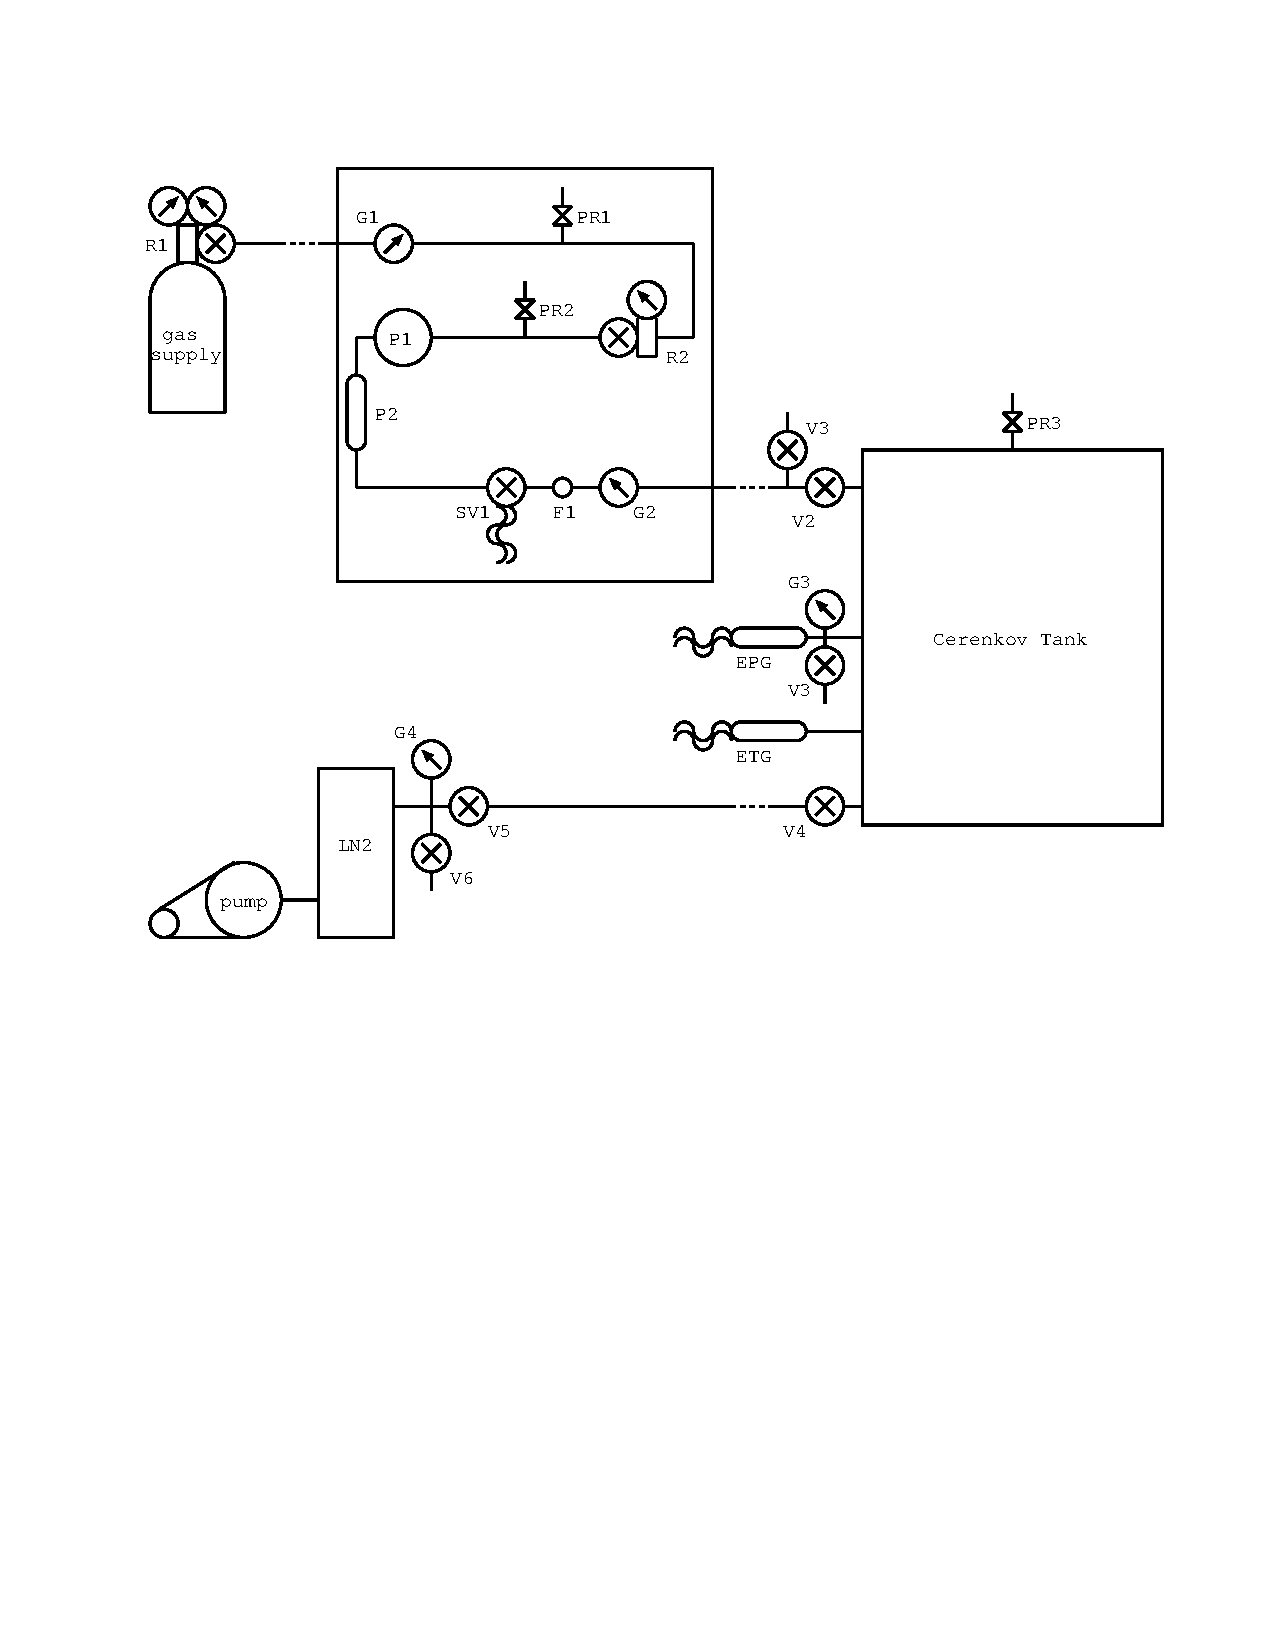
\includegraphics[height=5in,width=6in]{HMSgasC.pdf}
\caption{The Gas Handling System for the HMS \Cerenkov\ Detector. \label{fig:gas}}
\end{figure}

The HMS \Cerenkov\ Detector operates either as an e/$\pi$ or $\pi$/p
discriminator. Each mode has a unique set of procedures to prepare the tank
for operation. The nomenclature used in the description of these operation
procedures refers to Figure~\ref{fig:gas}, showing the gas handling system. Components 
shown
inside the dashed box of Figure~\ref{fig:gas}, are all located on the Gas Control Panel.

\paragraph{e/$\bf{\pi}$ Procedures}
For both e/$\bf{\pi}$ and p/$\bf{\pi}$ separation, the procedure 
has been to run with 0.4 to
0.9 (?) atmospheres of C4F10.  This is just a small modifiction to the
current p/pi procedures write-up described in the next section,
with the HMS running sub-atmospheric instead of supra-atmospheric. 

e/$\bf{\pi}$ running can also be accomplished using a nitrogen fill.
This mode of operation requires the tank to be filled with approximately
13.5~psia of $\rm{N_2}$.  The boiloff from the spectrometer magnets is a
perfect source of clean, dry Nitrogen, and is normally used to fill the
\Cerenkov\ tank.

Because the operating pressure is slightly subatmospheric, a pump and fill
procedure is employed.  First make sure that:
\begin{itemize}
\item The 40~mil windows are installed and oriented such that they curve
towards the interior of the tank.
\item Valves {\bf V1-V6} are closed.
\item The LN2 trap is filled.
\item There is enough oil in the pump.
\end{itemize}
The tank is now ready to be evacuated.
\begin{itemize}
\item Turn on the pump.
\item Slowly open {\bf V5}.  This evacuates the pump line.
\item Very slowly open {\bf V4}.  Since this valve connects the pump line to
the detector volume, the pump will work very hard.  Meter this valve
so that the pump is never under extreme stress.  It will take approximately
20~minutes to pump down the tank.
\end{itemize}
The tank can now be filled.
\begin{itemize}
\item Locate the boiloff manifold on the walkway on the top level of the
spectrometer, at the gap between Q3 and the dipole.
\item Turn the valve on this manifold open slightly so that the flow meter
barely registers a flow.
\item Connect the remaining end of the Tygon tubing to the vent of valve
{\bf V3} with a hose clamp.
\item Open valve {\bf V3}.
\item Increase the flow on the flow meter.  Do not exceed 100~cfpm.
\item When {\bf G3} or {\bf EPG} reach the operating pressure, close
the manifold valve.
\item Close {\bf V3}.
\end{itemize}
The fill should take approximately 30 minutes.  The detector should NEVER
be left unattended during a fill.  Frequently check the pressure in the tank
and be aware when the pressure nears one atmosphere.  DO NOT let the pressure
exceed one atmosphere under any circumstances; doing so risks damage to all of
the equipment and personnel in the detector hut.  This pump/fill procedure is usually 
repeated at least once to insure the
purity of the gas.

\paragraph{$\bf{\pi}$/p Procedures}
This mode of operation typically requires the tank to be filled with Freon-12
at pressures varying from 2 to 3~atm.  Because these operating pressures are
greater than 1~atm, the detector must be filled by dilution.  Contamination
from air, however, is not a major problem as the optical absorption properties
of air are actually more favorable than those of Freon-12 itself; the only
difficulty is the increase in pressure needed for a mixture of air and Freon
to achieve the same pion momentum threshold as for a pure sample of Freon.

First prepare the gas handling system:
\begin{itemize}
\item Make sure that the 60~mil windows are installed and oriented such that
they bulge outwards from interior of the tank.
\item Close the valves {\bf V2-V4}, and the valve on regulator {\bf R1}.
{\bf V1}, {\bf SV1}, and the valve on regulator {\bf R2} should be
open.
\item Open the valve on the gas supply bottle.
\item Adjust {\bf R1} to approximately 60 psig.
\item Open the valve on {\bf R1}.
\item Check to make sure gauge {\bf G1} agrees with the pressure setting
on {\bf R1}.
\item Adjust {\bf R2} so that a small flow is detected out the vent of
{\bf V1}.
\item Close {\bf V1}.
\item Adjust {\bf R2} to regulate at the required operating pressure.
\end{itemize}
The tank is now ready for the dilution process.  These steps should be
repeated as few times as possible to minimize the quantity of Freon-12 emitted
to the atmosphere.
\begin{itemize}
\item Record the tank pressure.
\item Open valve {\bf V2}.
\item Monitor the gas pressure until it reaches the required operating pressure.
NEVER let the pressure in the detector exceed 3~atmospheres.
\item Record the final pressure.
\item Open {\bf V3} to vent the tank.
\end{itemize}
From the recorded pressure readings, the threshold momentum of the mixture
of air and Freon-12 can be calculated (assuming the volume of the tank is
fixed).



\subsection{Lead Glass Shower Calorimeter}

The lead glass shower calorimeter consists of four stacks of
TF1 leaded glass (similar to SF1). Each stack contains thirteen
blocks for a total of 52 blocks. The blocks are 10 cm by 10 cm by 70
cm and all are read out by a PMT at one end at least.  Currently the
two layers have PMT readout at both ends.

High energy particles
emit Cerenkov radiation when passing through the glass and a signal
is collected that is proportional to the sum of the path lengths
travelled by all the
particles which are above the threshold for Cerenkov emission. High energy
electrons will produce a large signal as they have a large bremsstralung
cross section and the photons which are produced in the bremsstralung
process have a large cross section to produce electron positron pairs
(all of which will be above the Cerenkov threshold). This process
of bremsstralung followed by pair production is called an electromagnetic
shower.

The histograms associated with the calorimeter should be inspected
regularly to assure that it is functioning properly.

\section{Aerogel Detector}
The HMS Aerogel detector is located between the second wire chamber
and the first plane of the hodoscopes.
\sawnote{Does it take Positive HV.  If so note that fact in the Gas
  Cerenkov section.}
